% !TeX spellcheck = pt_BR
\documentclass[conference]{IEEEtran}

\ifCLASSINFOpdf
   \usepackage[pdftex]{graphicx}
\else
  % or other class option (dvipsone, dvipdf, if not using dvips). graphicx
  % will default to the driver specified in the system graphics.cfg if no
  % driver is specified.
  % \usepackage[dvips]{graphicx}
  % declare the path(s) where your graphic files are
  % \graphicspath{{../eps/}}
  % and their extensions so you won't have to specify these with
  % every instance of \includegraphics
  % \DeclareGraphicsExtensions{.eps}
\fi

\usepackage{amsmath}



% *** SUBFIGURE PACKAGES ***
%\ifCLASSOPTIONcompsoc
%  \usepackage[caption=false,font=normalsize,labelfont=sf,textfont=sf]{subfig}
%\else
%  \usepackage[caption=false,font=footnotesize]{subfig}
%\fi
% subfig.sty, written by Steven Douglas Cochran, is the modern replacement
% for subfigure.sty, the latter of which is no longer maintained and is
% incompatible with some LaTeX packages including fixltx2e. However,
% subfig.sty requires and automatically loads Axel Sommerfeldt's caption.sty
% which will override IEEEtran.cls' handling of captions and this will result
% in non-IEEE style figure/table captions. To prevent this problem, be sure
% and invoke subfig.sty's "caption=false" package option (available since
% subfig.sty version 1.3, 2005/06/28) as this is will preserve IEEEtran.cls
% handling of captions.
% Note that the Computer Society format requires a larger sans serif font
% than the serif footnote size font used in traditional IEEE formatting
% and thus the need to invoke different subfig.sty package options depending
% on whether compsoc mode has been enabled.
%
% The latest version and documentation of subfig.sty can be obtained at:
% http://www.ctan.org/pkg/subfig




% *** FLOAT PACKAGES ***
%
%\usepackage{fixltx2e}
% fixltx2e, the successor to the earlier fix2col.sty, was written by
% Frank Mittelbach and David Carlisle. This package corrects a few problems
% in the LaTeX2e kernel, the most notable of which is that in current
% LaTeX2e releases, the ordering of single and double column floats is not
% guaranteed to be preserved. Thus, an unpatched LaTeX2e can allow a
% single column figure to be placed prior to an earlier double column
% figure.
% Be aware that LaTeX2e kernels dated 2015 and later have fixltx2e.sty's
% corrections already built into the system in which case a warning will
% be issued if an attempt is made to load fixltx2e.sty as it is no longer
% needed.
% The latest version and documentation can be found at:
% http://www.ctan.org/pkg/fixltx2e


%\usepackage{stfloats}
% stfloats.sty was written by Sigitas Tolusis. This package gives LaTeX2e
% the ability to do double column floats at the bottom of the page as well
% as the top. (e.g., "\begin{figure*}[!b]" is not normally possible in
% LaTeX2e). It also provides a command:
%\fnbelowfloat
% to enable the placement of footnotes below bottom floats (the standard
% LaTeX2e kernel puts them above bottom floats). This is an invasive package
% which rewrites many portions of the LaTeX2e float routines. It may not work
% with other packages that modify the LaTeX2e float routines. The latest
% version and documentation can be obtained at:
% http://www.ctan.org/pkg/stfloats
% Do not use the stfloats baselinefloat ability as the IEEE does not allow
% \baselineskip to stretch. Authors submitting work to the IEEE should note
% that the IEEE rarely uses double column equations and that authors should try
% to avoid such use. Do not be tempted to use the cuted.sty or midfloat.sty
% packages (also by Sigitas Tolusis) as the IEEE does not format its papers in
% such ways.
% Do not attempt to use stfloats with fixltx2e as they are incompatible.
% Instead, use Morten Hogholm'a dblfloatfix which combines the features
% of both fixltx2e and stfloats:
%
% \usepackage{dblfloatfix}
% The latest version can be found at:
% http://www.ctan.org/pkg/dblfloatfix




% *** PDF, URL AND HYPERLINK PACKAGES ***
%
%\usepackage{url}
% url.sty was written by Donald Arseneau. It provides better support for
% handling and breaking URLs. url.sty is already installed on most LaTeX
% systems. The latest version and documentation can be obtained at:
% http://www.ctan.org/pkg/url
% Basically, \url{my_url_here}.




% *** Do not adjust lengths that control margins, column widths, etc. ***
% *** Do not use packages that alter fonts (such as pslatex).         ***
% There should be no need to do such things with IEEEtran.cls V1.6 and later.
% (Unless specifically asked to do so by the journal or conference you plan
% to submit to, of course. )

%\usepackage[brazilian]{babel}
%\usepackage[utf8]{inputenc}
%\usepackage[T1]{fontenc}
\usepackage{fancyhdr}


% correct bad hyphenation here
%\hyphenation{op-tical net-works semi-conduc-tor}


\pagestyle{fancy}
%\fancyhf{}
\chead{VII Workshop de P\'{o}s-Gradua\c{c}\~{a}o - Engenharia de Computa\c{c}\~{a}o - WPGEC 2018}
\renewcommand{\headrulewidth}{2pt}

\pagenumbering{gobble}

\begin{document}

\title{Bioclim - A Big Data reference architecture for Bioclimate data\\
	Bioclim - Uma arquitetura de refer\^{e}ncia de Big Data para dados bioclim\'{a}ticos}

\author{\IEEEauthorblockN{OLIVEIRA, R. M.\IEEEauthorrefmark{1};
CORR\^{E}A, P. L. P. G.\IEEEauthorrefmark{1}}
\IEEEauthorblockA{\IEEEauthorrefmark{1}PCS - Engenharia de Computa\c{c}\~{a}o e Sistemas Digitais - Universidade de S\~{a}o Paulo\\
	 E-mail: rmartine@usp.br, pedro.correa@usp.br}}


\maketitle

\thispagestyle{fancy}

\renewcommand{\abstractname}{Abstract}
\begin{abstract}
Abstract here.
\end{abstract}

\renewcommand\IEEEkeywordsname{Keywords}
\begin{IEEEkeywords}
\label{Keywords}
Biodiversity; Bioclimatic Data; GOAmazon; Big Data; Reference Architecture.
\end{IEEEkeywords}

\renewcommand{\abstractname}{Resumo}
\begin{abstract}
\label{Resumo}

\end{abstract}

\renewcommand\IEEEkeywordsname{Palavras-chave}
\begin{IEEEkeywords}
\label{Palavras-chave}
Biodiversidade; Dados Bioclim\'{a}ticos; GOAmazon; Arquitetura de Refer\^{e}ncia.
\end{IEEEkeywords}

\renewcommand\IEEEkeywordsname{Classifica\c{c}\~{a}o}
\begin{IEEEkeywords}
	\label{classificacao}
	Mestrado
\end{IEEEkeywords}

\renewcommand\IEEEkeywordsname{Categoria}
\begin{IEEEkeywords}
	\label{Categoria}
 	Iniciante
\end{IEEEkeywords}

\IEEEpeerreviewmaketitle

\section{Introdu\c{c}\~{a}o}
A busca por novos conhecimentos em bancos de dados n\~{a}o \'{e} algo recente\cite{Witten:2011}. No entanto, com o advento de Big Data, m\'{e}todos e algoritmos que trabalham na extra\c{c}\~{a}o de conhecimento precisam ser adaptados para lidar com grandes volumes de dados heterog\^{e}neos, que geralmente est\~{a}o imersos em um ambiente de \textit{Cloud Computing}, por causa de seu volume, e que pode receber novos dados em tempo real\cite{Crosas:2015}.

Pesquisadores de v\'{a}rios campos do conhecimento est\~{a}o dando aten\c{c}\~{a}o na  preserva\c{c}\~{a}o e reutiliza\c{c}\~{a}o de dados cient\'{i}ficos de suas pesquisas. Em vez de descartar os dados coletados, estes est\~{a}o sendo gerenciados, preservados e compartilhados por meio de reposit\'{o}rios especializados\cite{Fu:2017}.

Na busca pela constru\c{c}\~{a}o de reposit\'{o}rios especializados, existe a necessidade na comunidade cient\'{i}fica no que diz respeito ao provisionamento de informa\c{c}\~{o}es sobre biodiversidade, reunindo um conjunto de dados relacionados \`{a} ocorr\^{e}ncia de esp\'{e}cies animais e microrganismos registados nos herb\'{a}rios, museus, zoologia e sistemas microbianos, bem como dados de observa\c{c}\~{a}o e localiza\c{c}\~{a}o. A disponibilidade desta informa\c{c}\~{a}o poderia encorajar a investiga\c{c}\~{a}o no dom\'{i}nio da ci\^{e}ncia e tecnologia  na conserva\c{c}\~{a}o da biodiversidade, desenvolvimento sustent\'{a}vel e tamb\'{e}m como ferramenta de decis\~{a}o para a implementa\c{c}\~{a}o de pol\'{i}ticas governamentais que busquem preservar e restaurar a biodiversidade\cite{Peterson:2015}.

Atualmente vivemos em uma era onde os dados est\~{a}o em toda parte e dispon\'{i}veis a qualquer momento, da ordem de petabytes\cite{White:2015}. O aumento do volume de dados se deve a alguns fatores, tais como o poder de processamento dos computadores e o uso massivo de dispositivos m\'{o}veis e o baixo custo de armazenamento de dados em discos r\'{i}gidos\cite{Marquesone:2014}. Segundo White (2015), as redes sociais concentram o maior crescimento dos dados e a tendência é que em 2020 teremos produzido 44 zetabytes de dados.

No contexto de dados bioclim\'{a}ticos, h\'{a} alguns desafios no que diz respeito ao formato dos dados e por serem dados vindos de bases distintas. Temos dos dados de biodiversidade reposit\'{o}rios como o GBIF\cite{Gbif}, enquanto temos dos dados clim\'{a}ticos reposit\'{o}rios como o ARM\cite{ArmProject}. 

A proposta deste artigo \'{e} propor uma arquitetura de ref\^{e}rencia que.... %% FINALIZAR ESSE PARAGRAFO

% An example of a floating table. Note that, for IEEE style tables, the
% \caption command should come BEFORE the table and, given that table
% captions serve much like titles, are usually capitalized except for words
% such as a, an, and, as, at, but, by, for, in, nor, of, on, or, the, to
% and up, which are usually not capitalized unless they are the first or
% last word of the caption. Table text will default to \footnotesize as
% the IEEE normally uses this smaller font for tables.
% The \label must come after \caption as always.
%
%\begin{table}[!tp]
%% increase table row spacing, adjust to taste
%\renewcommand{\arraystretch}{1.3}
% if using array.sty, it might be a good idea to tweak the value of
% \extrarowheight as needed to properly center the text within the cells
%\caption{An Example of a Table}
%\label{table_example}
%\centering
%% Some packages, such as MDW tools, offer better commands for making tables
%% than the plain LaTeX2e tabular which is used here.
%\begin{tabular}{c|c}
%\hline
%\textbf{Number} & \textbf{Description} \\
%\hline
%Number 1 & Description 1 \\
%\hline
%Number 2 & Description 2\\
%\hline
%\end{tabular}
%\end{table}

\section{Justificativa}

Tais dados, quando na necessidade de serem analisados em grandes volumes para obten\c{c}\~{a}o de informa\c{c}\~{o}es precisas e pertinentes, precisam de ferramentas que possam se adequar \`{a} capacidade de dados a serem analisadas. N\~{a}o apenas ferramentas como tamb\'{e}m processos e metodologias que permitam a partir de uma base de dados de grande volume realizar uma an\'{a}lise efetiva do conjunto de dados, trazendo uma visualiza\c{c}\~{a}o mais precisa do conjunto de dados

\section{Metodologia}
O Objetivo da arquitetura proposta \'{e} permitir manipular dados bioclim\'{a}ticos em estruturas l\'{o}gicas separadas, por\'{e}m utilizando a mesma estrutura f\'{i}sica, utilizando recursos computacionais compartilhados atrav\'{e}s da Computa\c{c}\~{a}o em Nuvem. A arquitetura ser\'{a} baseada na arquitetura de refer\^{e}ncia da Fig. \ref{ref_arch}\cite{Hashem:2015}.

\begin{figure}[!tp]
	\centering
	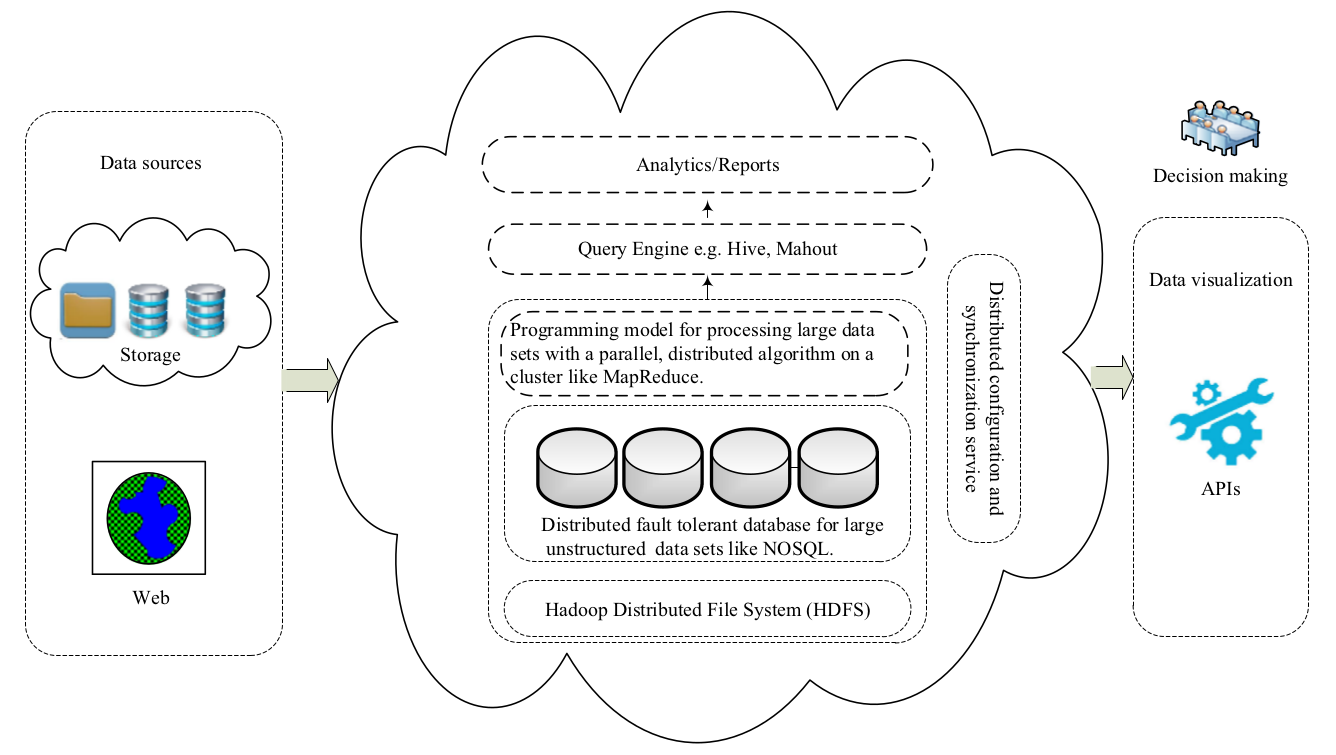
\includegraphics[width=2.5in]{big-data-computing.png}
	% where an .eps filename suffix will be assumed under latex, 
	% and a .pdf suffix will be assumed for pdflatex; or what has been declared
	% via \DeclareGraphicsExtensions.
	\caption{Arquitetura de Referencia}
	\label{ref_arch}
\end{figure}

De acordo com o diagrama, todo o fluxo de an\'{a}lise \'{e} gerenciado pela infraestrura em nuvem de forma a automatizar a implanta\c{c}\~{a}o dos diversos componentes que comp\~{o}em a arquitetura. Um Sistema de Arquivos compartilhado \'{e} utilizado para armazenar todos os dados n\~{a}o-estruturados e semi-estruturados (o chamado Data Lake) para que assim a camada de MapReduce converta os dados para assim armazenar em uma camada de dados estruturados, definido como o Banco de Dados NoSQL. Uma ferramenta de an\'{a}lise e relat\'{o}rio \'{e} utilizada para realizar a an\'{a}lise explorat\'{o}ria dos dados e assim obter mais conhecimento sobre os dados estruturados. Para alimentar a camada de an\'{a}lise e relat\'{o}rio, teremos uma camada de consulta para trazer os dados. Toda a arquitetura \'{e} suportada por um mecanismo de configura\c{c}\~{a}o e sincroniza\c{c}\~{a}o para gerenciar e monitorar toda a infraestrutura de fluxo dos dados. Ap\'{o}s toda a execu\c{c}\~{a}o do fluxo de dados, uma ferramenta de visualiza\c{c}\~{a}o de dados \'{e} usada para oferecer uma an\'{a}lise explanat\'{o}ria dos dados de forma a criar um Dashboard com as conclus\~{o}es feitas sobre os dados.

Uma das grandes vantagens dessa arquitetura \'{e} a utiliza\c{c}\~{a}o de plataforma de Computa\c{c}\~{a}o em Nuvem para oferecer recursos computacionais para a arquitetura proposta de forma el\'{a}stica, sob demanda e autom\'{a}tica. A proposta desse artigo \'{e} realizar um experimento com dados do GOAmazon e utilizando a plataforma Internuvem da USP para fornecer ma\'{a}quinas virtuais em um ambiente de Computa\c{c}\~{a}o em Nuvem de forma a provisionar todos os servi\c{c}os exigidos para a implementa\c{c}\~{a}o da arquitetura. Para a camada de gerenciamento da arquitetura, a plataforma de Computa\c{c}\~{a}o em Nuvem ser\'{a} baseada em containers, trazendo assim maior granularidade para a plataforma. Como o experimento ser\'{a} baseado nos dados da campanha GOAmazon, organizada por diversas institui\c{c}\~{o}es (dentre elas o ARM\cite{ArmProject}), consultamos o grupo para entender a forma como suportar esses dados. Sendo assim, os dados brutos vindos do ARM ser\~{a}o armazenados em um sistema de arquivos compartilhado e de alto desempenho, e assim processados atrav\'{e}s de um mecanismo executado com o Apache Spark\cite{ApacheSpark} para assim armazenar os dados no servidor NoSQL Cassandra\cite{ApacheCassandra}. Uma vez que o Apache Spark consiste em uma infraestrutura relativamente complexa de provisionar tanto em ambientes de Computa\c{c}\~{a}o em Nuvem quando em servidores f\'{i}sicos, a cria\c{c}\~{a}o e monitoramento dessa infraestrutura ser\'{a} delegada \`{a} ferramenta RADAnalytics.io\cite{RadanalyticsIo}. Enfim, a arquitetura oferecer\'{a} suporte ao desenvolvimento nas linguagens Java, Scala, Python e R e o suporte ao Apache Zeppelin\cite{ApacheZeppelin} como ferramenta para Visualiza\c{c}\~{a}o de Dados.

\begin{figure}[!tp]
	\centering
	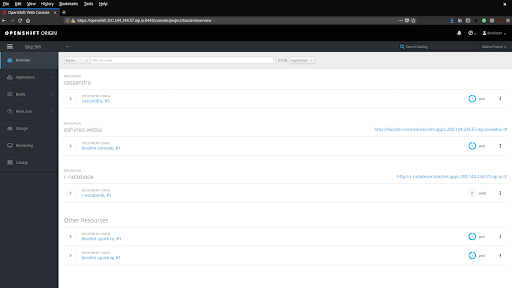
\includegraphics[width=2.5in]{bioclim.png}
	% where an .eps filename suffix will be assumed under latex, 
	% and a .pdf suffix will be assumed for pdflatex; or what has been declared
	% via \DeclareGraphicsExtensions.
	\caption{Interface de gerenciamento da arquitetura}
	\label{bioclim}
\end{figure}

For the first phase of this architecture, we provisioned a Virtual Machine in the USP internuvem platform with 2vCPUS and 4GB of RAM, attached to a public IP where we can make use of external access to access the infrastructure on the Internet. On top of this Virtual Machine we deployed an all-in-one OpenShift environment to deploy the initial components for the Bioclim platform, based on containers to provide better use of the limited compute resource for the Virtual Machine. After deploying successfully an OpenShift platform, the RADAnalytics.io is deployed on top of the OpenShift platform and the Apache Spark cluster was provisioned. Again, as the Virtual Machine is very limited in resources the Apache Spark cluster is deployed with a single master and a single worker.


\section{Resultados Esperados}

Ao fim dos experimentos, espera-se que uma arquitetura de refer\^{e}ncia seja proposta de forma a tratar especificamente de dados bioclim\'{a}ticos e trazendo ganho de processamento em menor tempo.

\bibliographystyle{abntex2-num}
\bibliography{template}

\end{document}


